\chapter{Proposed System Architecture}
\section{Introduction}
This chapter represents the methodology used in the development of the Voice Search Chrome Extension. The chapter focuses on the design, workflow and the core functionalities of the proposed system. This system enables users to control the browser for several facilities like search in the internet, form fill up, read the selected content and click the highlighted links through voice commands.

The methodology demonstrates modularity, scalability and user-friendliness. This system is divided into different logical components to ensure the accurate speech recognition and identify the correct command by parsing and executing the right operation. This chapter describes the architecture, workflow and features through diagrams, flowcharts and algorithm to make it easy to understand the system properly.

\section{System Architecture}
\section*{Overview of Components}
\begin{itemize} 
\item \textbf{User Interface Module:} Provides a floating microphone button for capturing voice input.
\item \textbf{Speech Recognition Module:} Converts spoken words into text using the browser’s Web Speech API.
\item \textbf{Command Processing Module:} Detects the language and identifies the user’s intent by matching text with predefined commands stored in JSON files (en.json, bn.json).
\item \textbf{Action Execution Module:} Performs the requested browser actions, including tab control, scrolling, inline search, media handling, link clicking, and form filling.
\item \textbf{Feedback Module:} Provides visual or audio feedback to the user, such as highlighting text during read-aloud or confirming executed actions.
\end{itemize}

\begin{figure}[H]
   \centering
   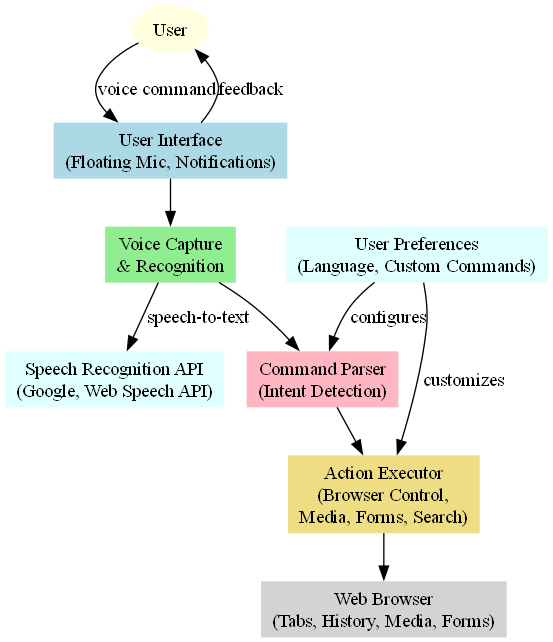
\includegraphics[width=4in]{latex/Chap3/system_architecture.png}
   \caption{Architecture of the Voice Search Extension}
   \label{fig:model}
\end{figure}
Figure 3.1 illustrates the overall architecture of the Voice Search Extension, highlighting the interaction between the user, the system modules, and the browser environment.


\section{System Workflow}
\subsection{Functional Flow}
Functional Flow describes the steps how total process keeps forward from start to end. This flow starts when user activates the microphone by click. Then speech is captured, speech-to-text translation, intent parsing and then mapped to the correct actions. The flow ends with the execution of the action and followed by feedback through voice transcript or audio feedback.
Figure 3.2: Functional Flow of Voice Command Processing illustrates this sequence.

\begin{figure}[H]
   \centering
   \includegraphics[height=4in]{latex/Chap3/Flow-diagram.png}
   \caption{Functional Flow Diagram of the proposed system}
   \label{fig:flow-diagram}
\end{figure}
 
\subsection{User Interactions and Use Cases}
This system supports different interaction between users. Some are: Hands free web search, inline online search on google, youtube or wikipedia, media playback control, read-loud functionality on any webpage on both English or Bangla, click highlighted links, voice controlled form filling, browser control like switching tabs, auto scrolling, open/close tabs.

These use cases are represented in Figure 3.3.
Figure 3.3 illustrates the different ways the user interacts with the extension, including search, media control, form filling, navigation, and text-to-speech reading.

\begin{figure}[H]
   \centering
   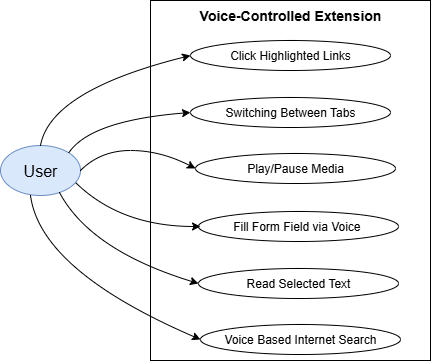
\includegraphics[width=4in]{latex/Chap3/User-Cases-Diagram.png}
   \caption{User-cases diagram of voice controlled system}
   \label{fig:usr-cases-diagram}
\end{figure}


\subsection{Data Organization and Relationships}
Voice input, commands, actions, preference, language are organized follows a structured model in a way that it links natural voice input with the executable commands in action. For example “search python tutorials for beginners” maps to the Search Handler with the site to visit and query.

Figure 3.4: Data Structure and Relationships illustrates this organization.It depicts how commands, actions, and user preferences are organized in the system. Spoken input is first recognized and mapped into intents with associated parameters. User Preferences such as language, zoom level, reading speed modify both interpretation and execution. Finally mapped commands are executed as system action to interact with browser.

 \begin{figure}[H] 
   \centering
   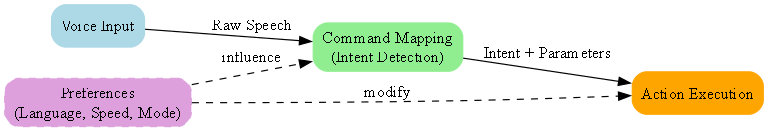
\includegraphics[width=6in]{latex/Chap3/data_structure_diagram.png}
   \caption{Data Relationship Diagram Among Components}
   \label{fig:model}
\end{figure}

\bigskip
\bigskip
\bigskip

\section{Demonstration and Illustration}
The extension’s usability is demonstrated through:

\begin{figure}[ht]
   \centering
   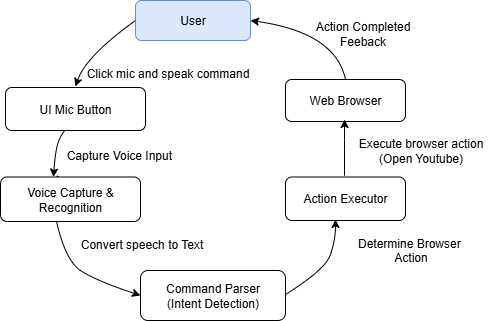
\includegraphics[width=5.5in]{latex/Chap3/sequence-diagram.png}
   \caption{Sequence diagram with detailed workflow }
   \label{fig:model}
\end{figure}
This sequence diagram presents the detailed step-by-step message flow between elements for single command execution.

\begin{itemize}
\item The process initiates while user click on mic and speak any command.
\item	UI mic button captures the voice input and pass through it to the Voice Capture \& Recognition component.
\item This component converts speech into text and transfer it to the Command Parser.
\item Command Parser detect the intent by parsing the text and transfer appropriate browser action to the action executor section. 
\item Action Executor Component executes the browser action in web browser such as inline search in YouTube shown in above figure. 
\item Web browser then send the feedback to the user by displaying the output.
\end{itemize}

\section{Algorithmic Approach For Implementing Features}
In this section, different feature modules are described along with algorithms which show how each feature can be implemented. The implementation process with code is discussed in Chapter 4 for each feature.

\subsection{Capturing and Interpreting Voice Commands}
This subsection describes how to capture and interpret voice commands spoken by users. \texttt{Algorithm 1} describes the way of  processing of a voice command from capture to execution. Speech Recognition API is used here to detect text from speech. If intent matches with commands, it executes actions otherwise provides error message to user.

\begin{algorithm}[H] 
    \caption{Voice Command Processing from capturing to execution}
    \label{alg:voice_command_processing}
    \textbf{Input:} voice\_input
    \textbf{Output:} executed\_action
    \begin{algorithmic}[1] % The [1] option enables line numbering
        \State Capture \Call{voice\_input}{} from microphone
        \State Convert \Call{voice\_input}{} to text using Speech Recognition API
        \State Detect language of text
        \If {intent matches known command}
            \State Execute corresponding action
        \Else
            \State Provide error/feedback to user
        \EndIf
        \State \Return executed\_action
    \end{algorithmic}
\end{algorithm}


\subsection{Media Playback and Sound Management}

This feature allows the user to control media playback (play, pause, volume, mute, forward, backward) using voice commands. \texttt{Algorithm 2} describes how intent is detected and how associated video content is manipulated in the DOM.

\begin{algorithm}[H]
    \caption{Media Playback and Sound Management}
    \label{alg:media_control}
    \textbf{Input:} voice\_command  
    \textbf{Output:} media\_state\_changed  
    \begin{algorithmic}[1]
        \State Capture voice command
        \State Convert to text and extract intent
        \If {intent = "play"} 
            \State Execute \Call{video.play}{} 
        \ElsIf {intent = "pause"} 
            \State Execute \Call{video.pause}{} 
        \ElsIf {intent = "volume up"} 
            \State Increase volume by 10\% 
        \ElsIf {intent = "volume down"} 
            \State Decrease volume by 10\% 
        \ElsIf {intent = "forward/backward"} 
            \State Adjust \Call{video.currentTime}{} by given seconds 
        \EndIf
        \State Provide feedback to user
    \end{algorithmic}
\end{algorithm}

\subsection{Tab Navigation and Switching}

This feature allows the user to manage tab navigation(open, close, or switch browser tabs) by voice commands.\texttt{Algorithm 3} refers how tab-related intent are matched and then sends a message to Chrome’s API to perform the related action.

\begin{algorithm}[H]
    \caption{Tab Navigation and Switching}
    \label{alg:tab_management}
    \textbf{Input:} voice\_command  
    \textbf{Output:} tab\_action\_executed  
    \begin{algorithmic}[1]
        \State Capture voice command
        \State Convert to text and detect tab intent
        \If {intent = "open site"} 
            \State Extract site name and call \Call{chrome.tabs.create}{url} 
        \ElsIf {intent = "close tab"} 
            \State Call \Call{chrome.tabs.remove}{currentTab} 
        \ElsIf {intent = "switch tab"} 
            \State Identify target tab and call \Call{chrome.tabs.update}{active=true} 
        \EndIf
        \State Confirm action with visual/audio feedback
    \end{algorithmic}
\end{algorithm}



\subsection{Page View Adjustment via Voice-Controlled Scrolling and Zooming}

This feature lets the user scroll or zoom in webpage with voice commands. \texttt{Algorithm 4} describes the step by step process for mapping commands to page events like window scroll or zoom adjustment.

\begin{algorithm}[H]
    \caption{Scrolling and Zooming Process}
    \label{alg:scroll_zoom}
    \textbf{Input:} voice\_command  
    \textbf{Output:} adjusted_page_view  
    \begin{algorithmic}[1]
        \State Capture voice command
        \State Convert to text and detect scroll/zoom intent
        \If {intent = "scroll up"} 
            \State Execute \Call{window.scrollBy}{} by X pixels to top
        \ElsIf {intent = "scroll down"} 
            \State Execute \Call{window.scrollBy}{} by X pixels to bottom
        \ElsIf {intent = "zoom in"} 
            \State Increase \Call{document.body.style.zoom}{} by 10\% 
        \ElsIf {intent = "zoom out"} 
            \State Decrease \Call{document.body.style.zoom}{} by 10\% 
        \EndIf
        \State Provide feedback bubble to confirm change
    \end{algorithmic}
\end{algorithm}

\subsection{Link Highlighting and Selection}

This feature allows the user to highlight, hide, or click web page links using voice commands. All visible links are numbered, and the user can refer to them by spoken numbers or partial text are described in \texttt{Algorithm 5}.

\begin{algorithm}[H]
    \caption{Link Highlighting and Selection}
    \label{alg:link_interaction}
    \textbf{Input:} voice\_command  
    \textbf{Output:} link\_highlighted/clicked  
    \begin{algorithmic}[1]
        \State Capture voice command
        \State Convert to text and detect link intent
        \If {intent = "show links"} 
            \State Highlight all links with numeric labels
        \ElsIf {intent = "hide links"} 
            \State Remove all link overlays
        \ElsIf {intent = "click link"} 
            \If {value is number} 
                \State Click link by index 
            \Else 
                \State Find link by matching title text and click 
            \EndIf
        \EndIf
        \State Provide feedback about clicked link
    \end{algorithmic}
\end{algorithm}

\vspace{1in}

\subsection{Text-to-Speech Conversion with highlighted sentence}

This feature enables the user to listen to web page text read aloud.\texttt{Algorithm 6} describes how the system detects the selected text, highlights it sentence by sentence, and uses the speech synthesis API to read it loudly.

\begin{algorithm}[H]
    \caption{Reading Selected Text Process}
    \label{alg:read_text}
    \textbf{Input:} selected\_text  
    \textbf{Output:} audio\_narration  
    \begin{algorithmic}[1]
        \State Detect if text is selected on webpage
        \If {selection is empty} 
            \State Provide error feedback 
        \Else 
            \State Pass selected text to \Call{SpeechSynthesis}{}
            \State Highlight sentence sequentially during reading
            \State Auto-scroll page along with reading
        \EndIf
    \end{algorithmic}
\end{algorithm}


\subsection{Voice Controlled Inline Search Execution }

\texttt{Algorithm 7} demonstrates how the system performs inline search without opening a new tab(Google, YouTube). At first it clears the input, insert the query, then submit the query to display the output.

\begin{algorithm}[H] 
    \caption{Inline Search}
    \label{alg:inline_search}
    \textbf{Input:} query, active\_tab
    \textbf{Output:} search\_results
    \begin{algorithmic}[1]
        \State Check if \textbf{active\_tab} supports inline search
        \State Clear current search input
        \State Insert \textbf{query} into search box
        \State Press Enter to display results
        \State Highlight first search result (optional)
    \end{algorithmic}
\end{algorithm}

\subsection{System Response Time}
In this subsection, an equation is presented to calculate the total time taken from the capture of the voice input to perform execution.
\vspace{.5in}

\begin{equation}
T_{response} = T_{capture} + T_{recognition} + T_{parsing} + T_{execution}
\end{equation}
\begin{align*}
T_{\text{Response}} &= \text{Time taken from input to execute the action.} \\
T_{\text{Capture}} &= \text{Time to capture voice input} \\
T_{\text{Recognition}} &= \text{Time for speech-to-text conversion} \\
T_{\text{Parsing}} &= \text{Time to parse command and determine intent} \\
T_{\text{Execution}} &= \text{Time to execute the browser action}
\end{align*}

\section{Scalability and Extensibility}
The modular design of this system enables to add new commands and services(like Google Doc voice typing).The design of the system makes this scalable and extensive to new features. It can support to a new language commands by adding them in new JSON file. In future it is possible to add NLP features for more natural speech interpretation and reduce response time. 
\section{Conclusion}
This chapter presents the architecture, workflow of the voice based chrome extension. This system is modular, scalable and user-friendly by enabling voice command inclusion. Algorithms and diagrams clarify the step by step system design and its workflow from user input to actions. 
This proposed methodology provides a solid foundation to design, develop and testing the system and also its future enhancement by adding new features and including new languages.






